\documentclass{beamer}
\usetheme{metropolis}
\usepackage{graphicx}
\usepackage{diagbox}
\usepackage{tcolorbox}
\title{Computer Logic and Digital Circuit Design (PHYS306/COSC330): Unit 4}
\author{Jordan Hanson}
\institute{Whittier College Department of Physics and Astronomy}

\begin{document}
\maketitle

\section{Summary}

\begin{frame}{Unit 4 Summary}
\begin{enumerate}
\item Analog to Digital Conversion (ADC)
\item Digital to Analog Conversion (DAC)
\item Digital Signal Processing (DSP)
\item Digital Signal Processors
\end{enumerate}
\end{frame}

\begin{frame}{Analog to Digital Conversion}
\begin{figure}
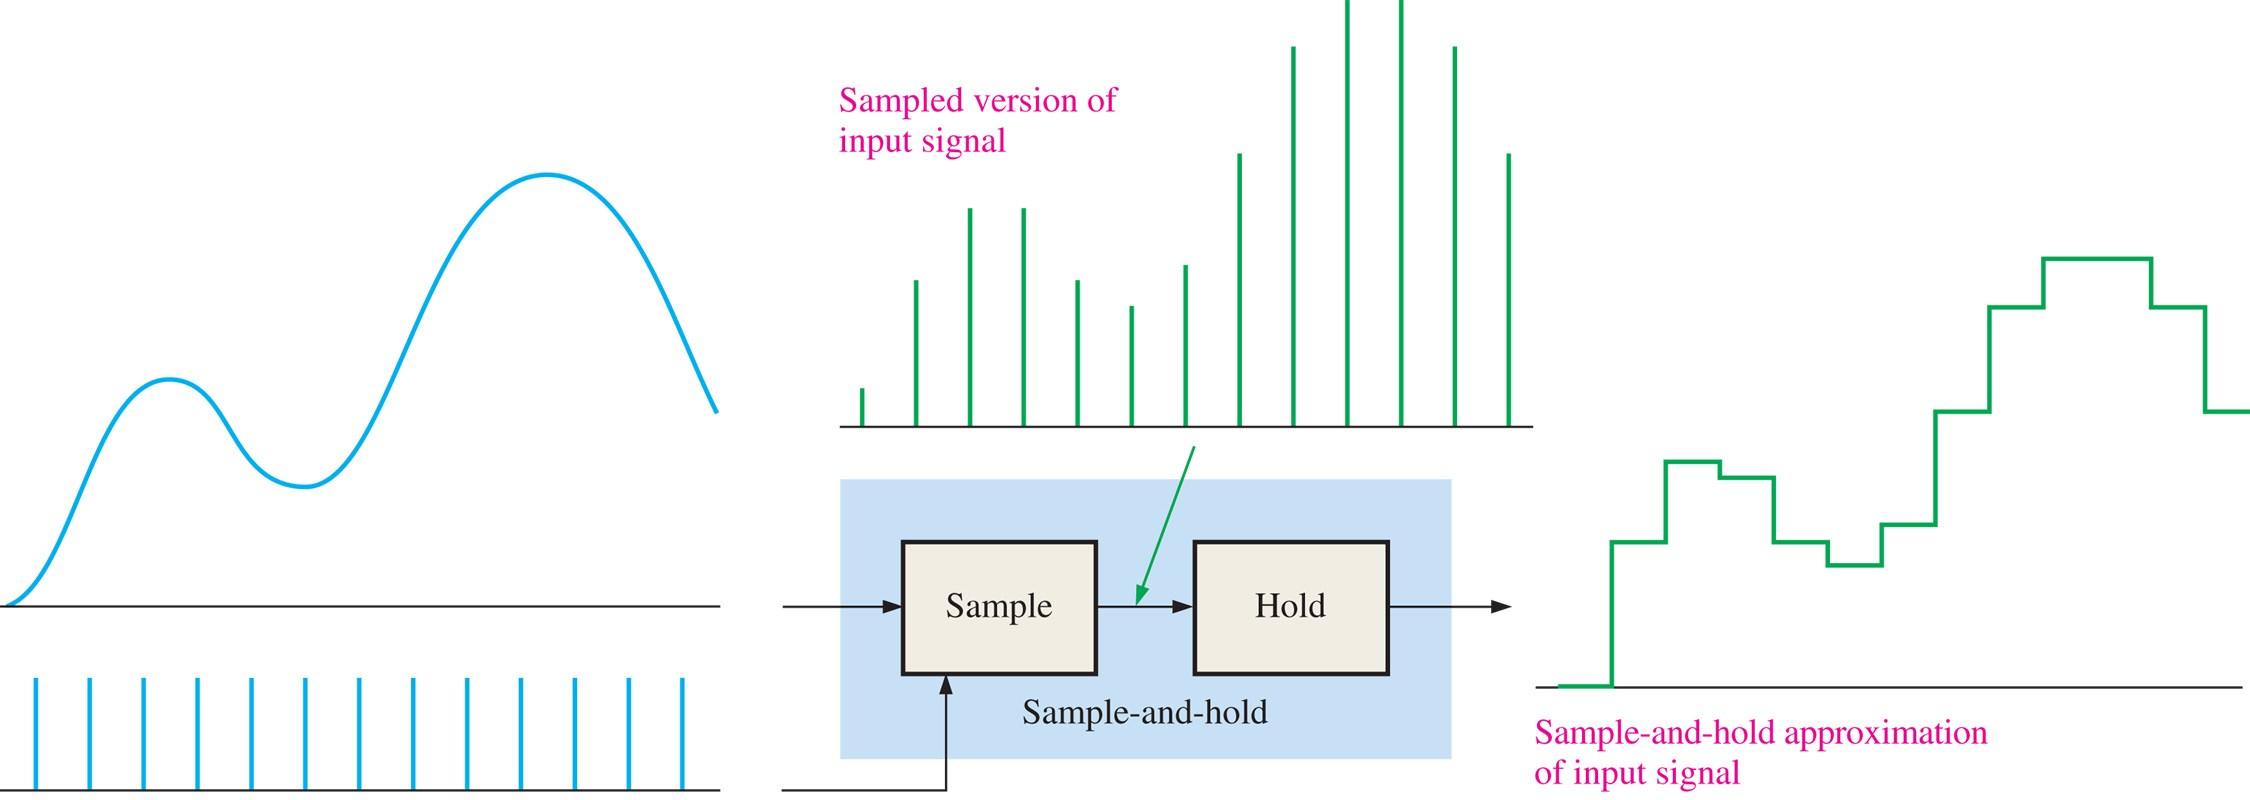
\includegraphics[width=0.75\textwidth]{figures/adc_1.jpg} \\ \vspace{1cm}
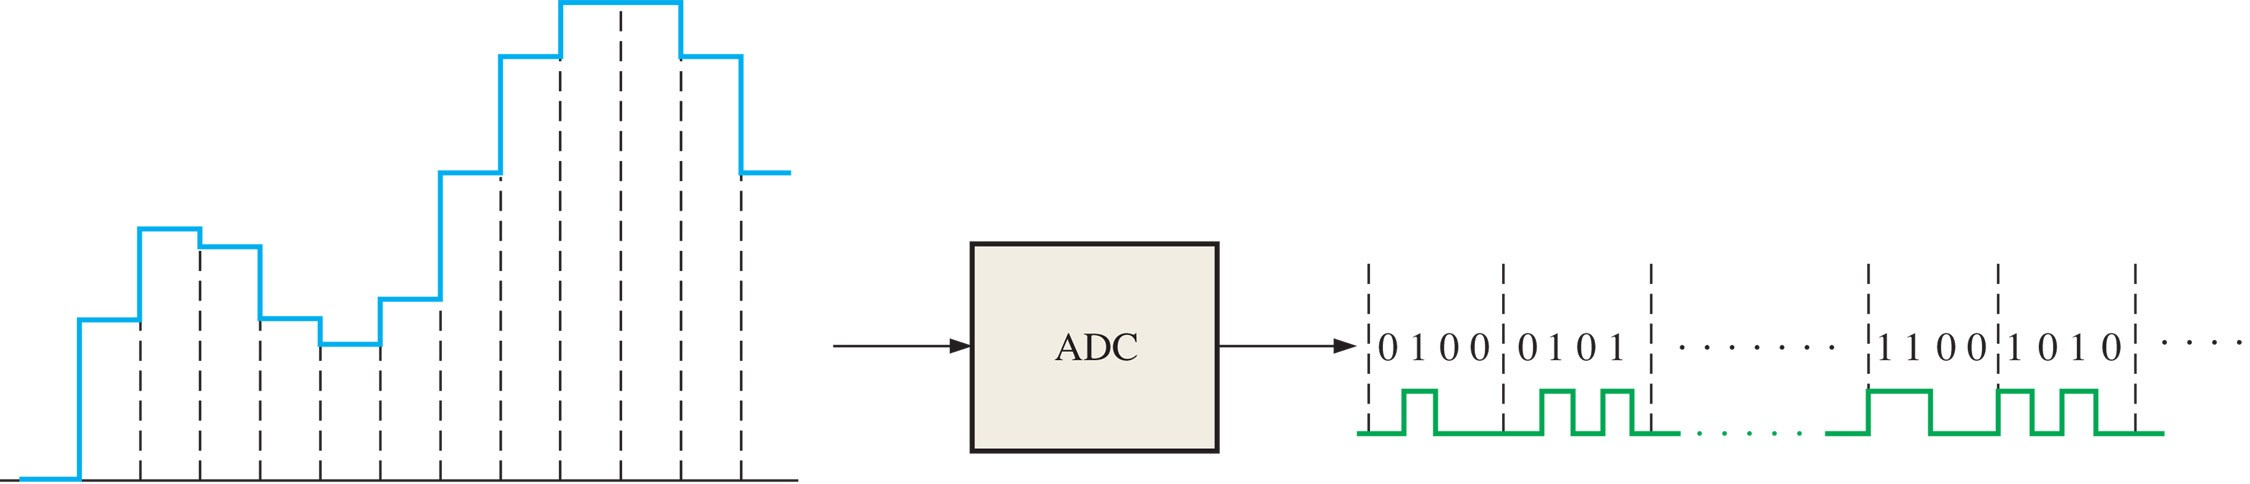
\includegraphics[width=0.75\textwidth]{figures/adc_2.jpg}
\caption{\label{fig:1} (Top) Analog signal being converted to digital data via sample and hold. (Bottom) Coded output.}
\end{figure}
\end{frame}

\begin{frame}{Analog to Digital Conversion}
\begin{figure}
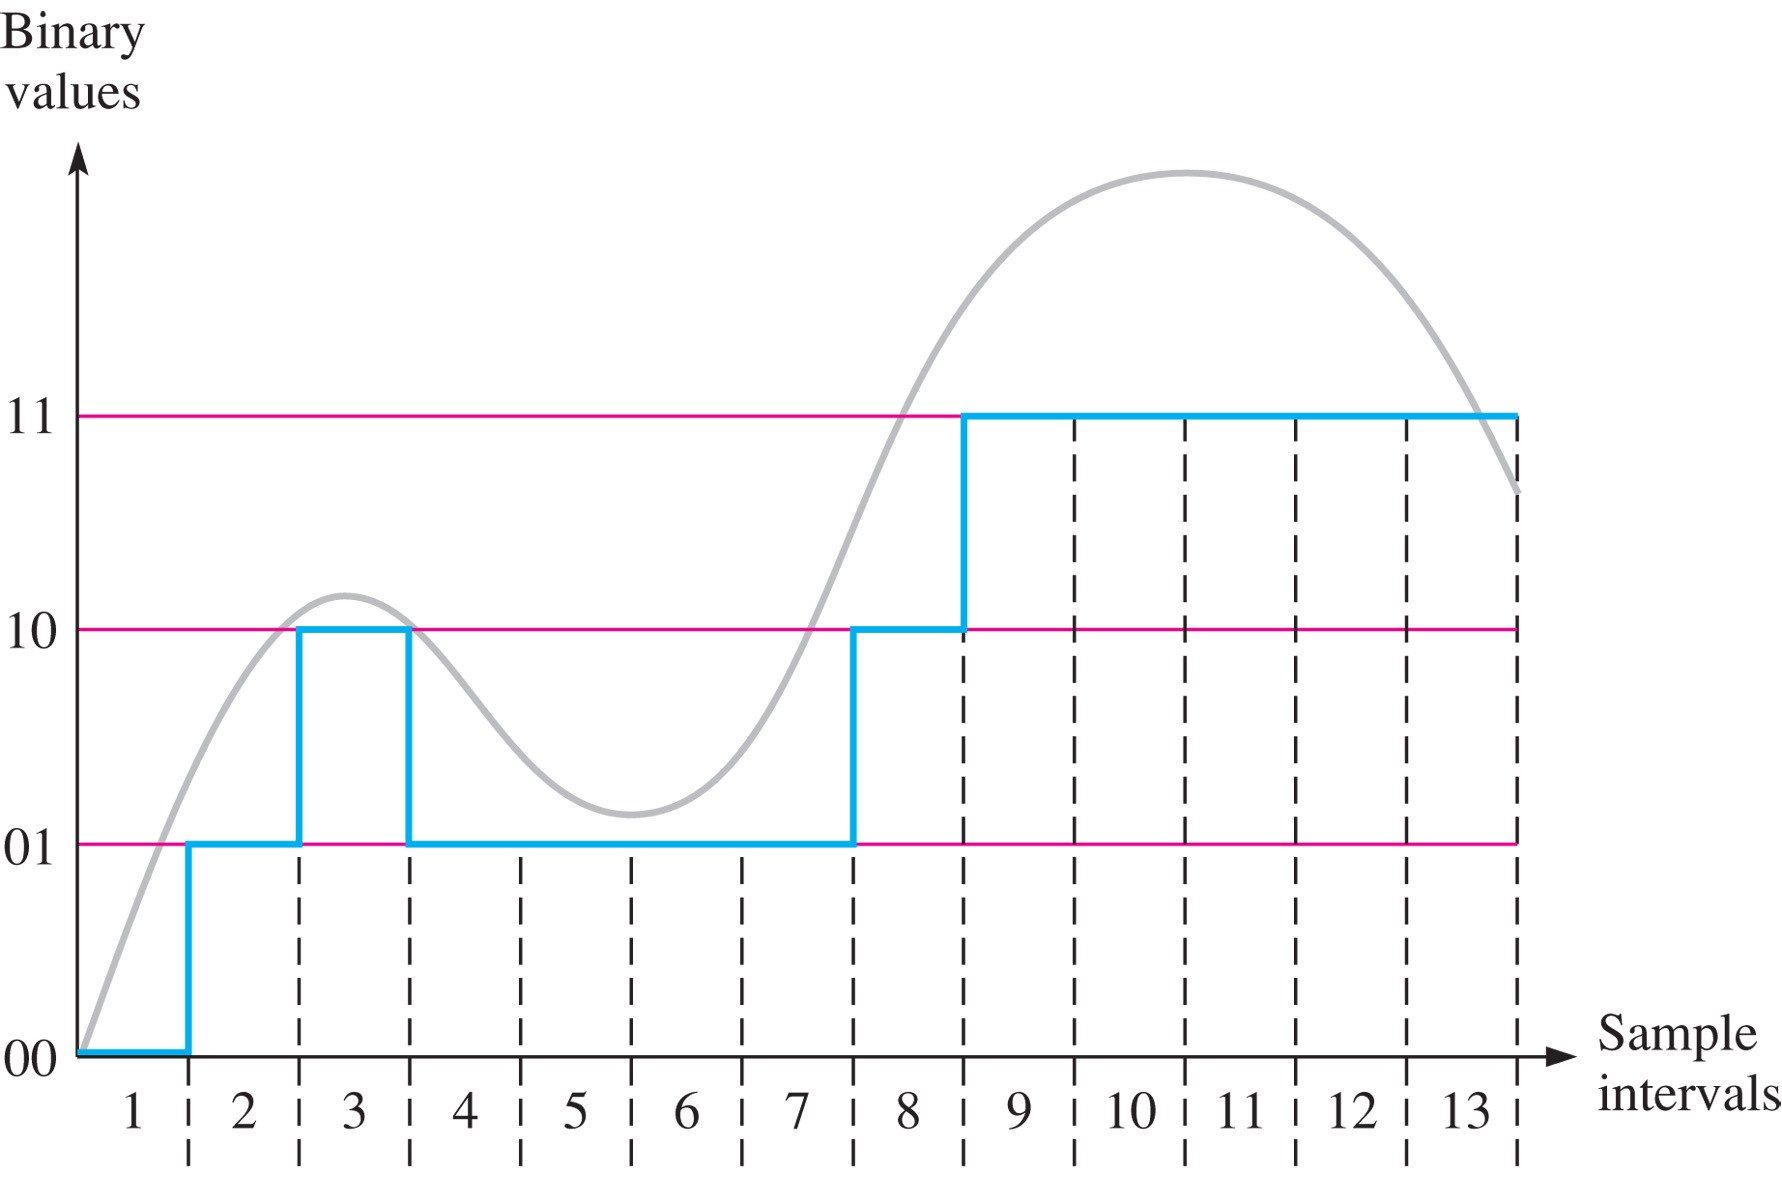
\includegraphics[width=0.45\textwidth]{figures/adc_3.jpg} \hspace{1cm}
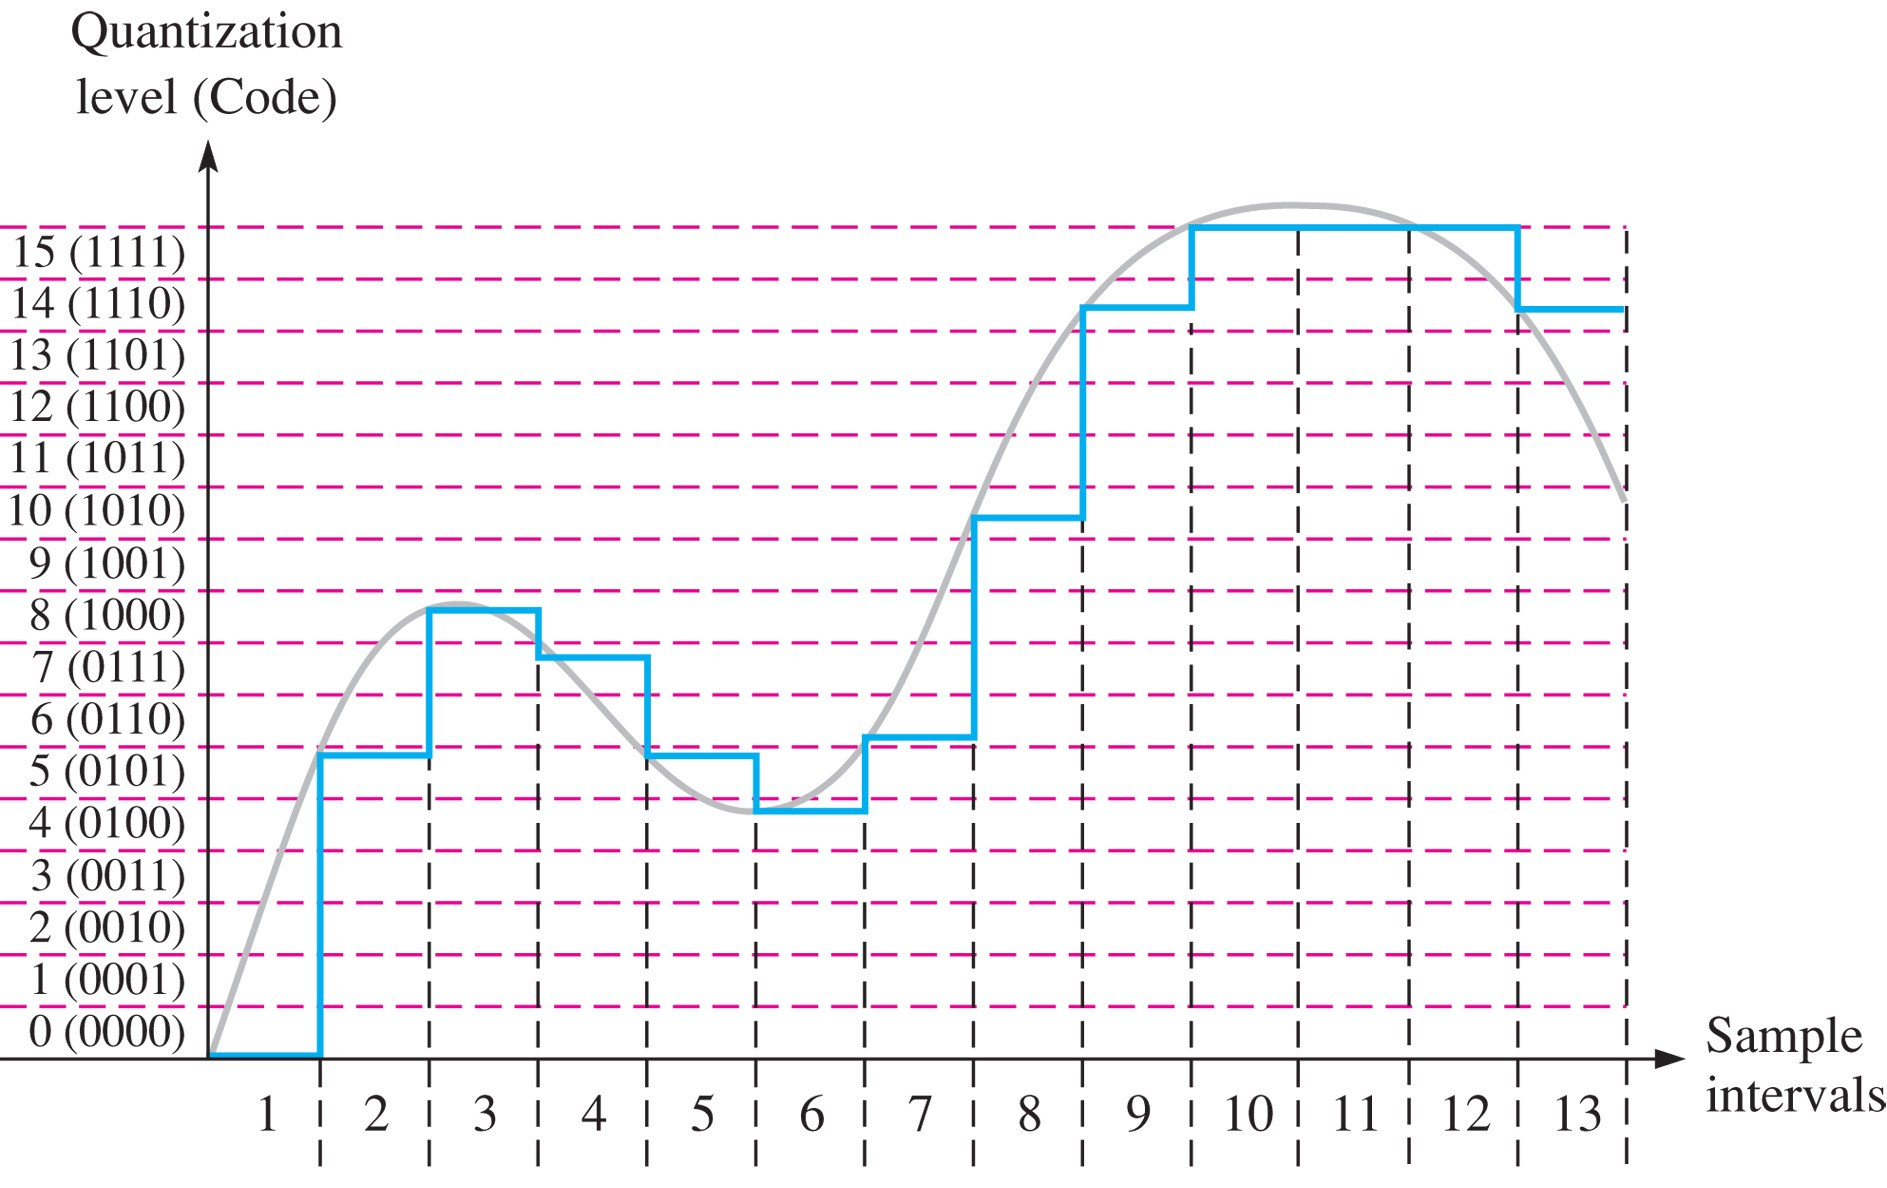
\includegraphics[width=0.45\textwidth]{figures/adc_4.jpg}
\caption{\label{fig:2} (Top) 3-bit conversion. (Bottom) 4-bit conversion.}
\end{figure}
\end{frame}

\begin{frame}{Analog to Digital Conversion}
\begin{figure}
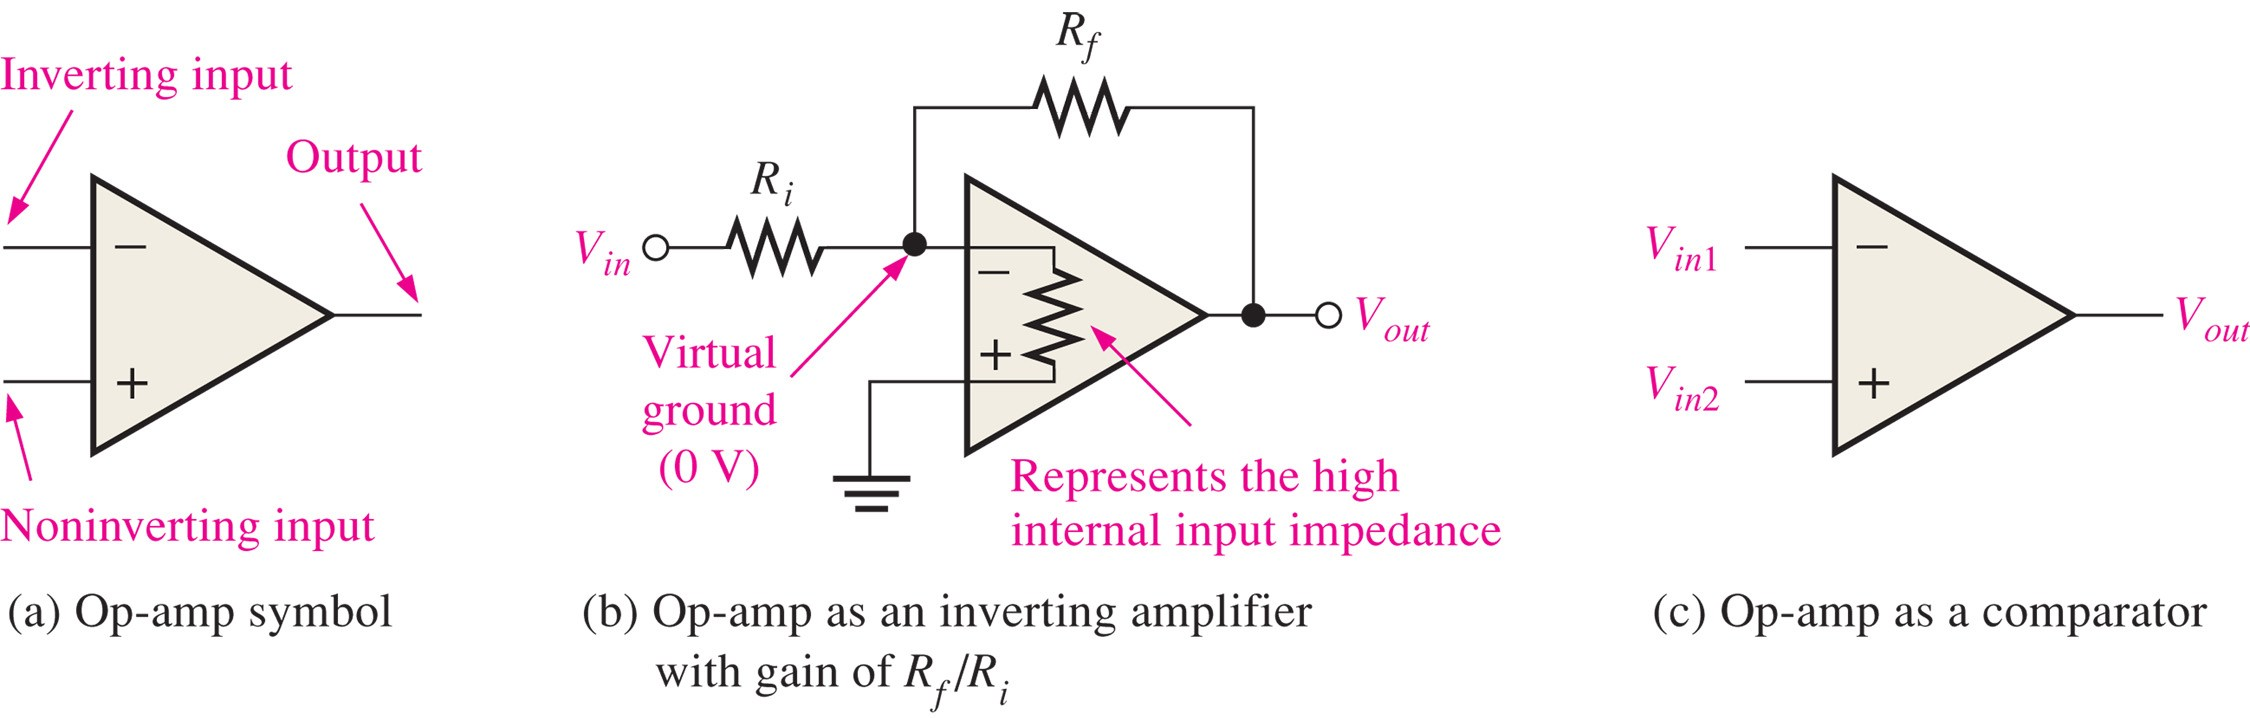
\includegraphics[width=0.55\textwidth]{figures/adc_5.jpg} \hspace{1cm}
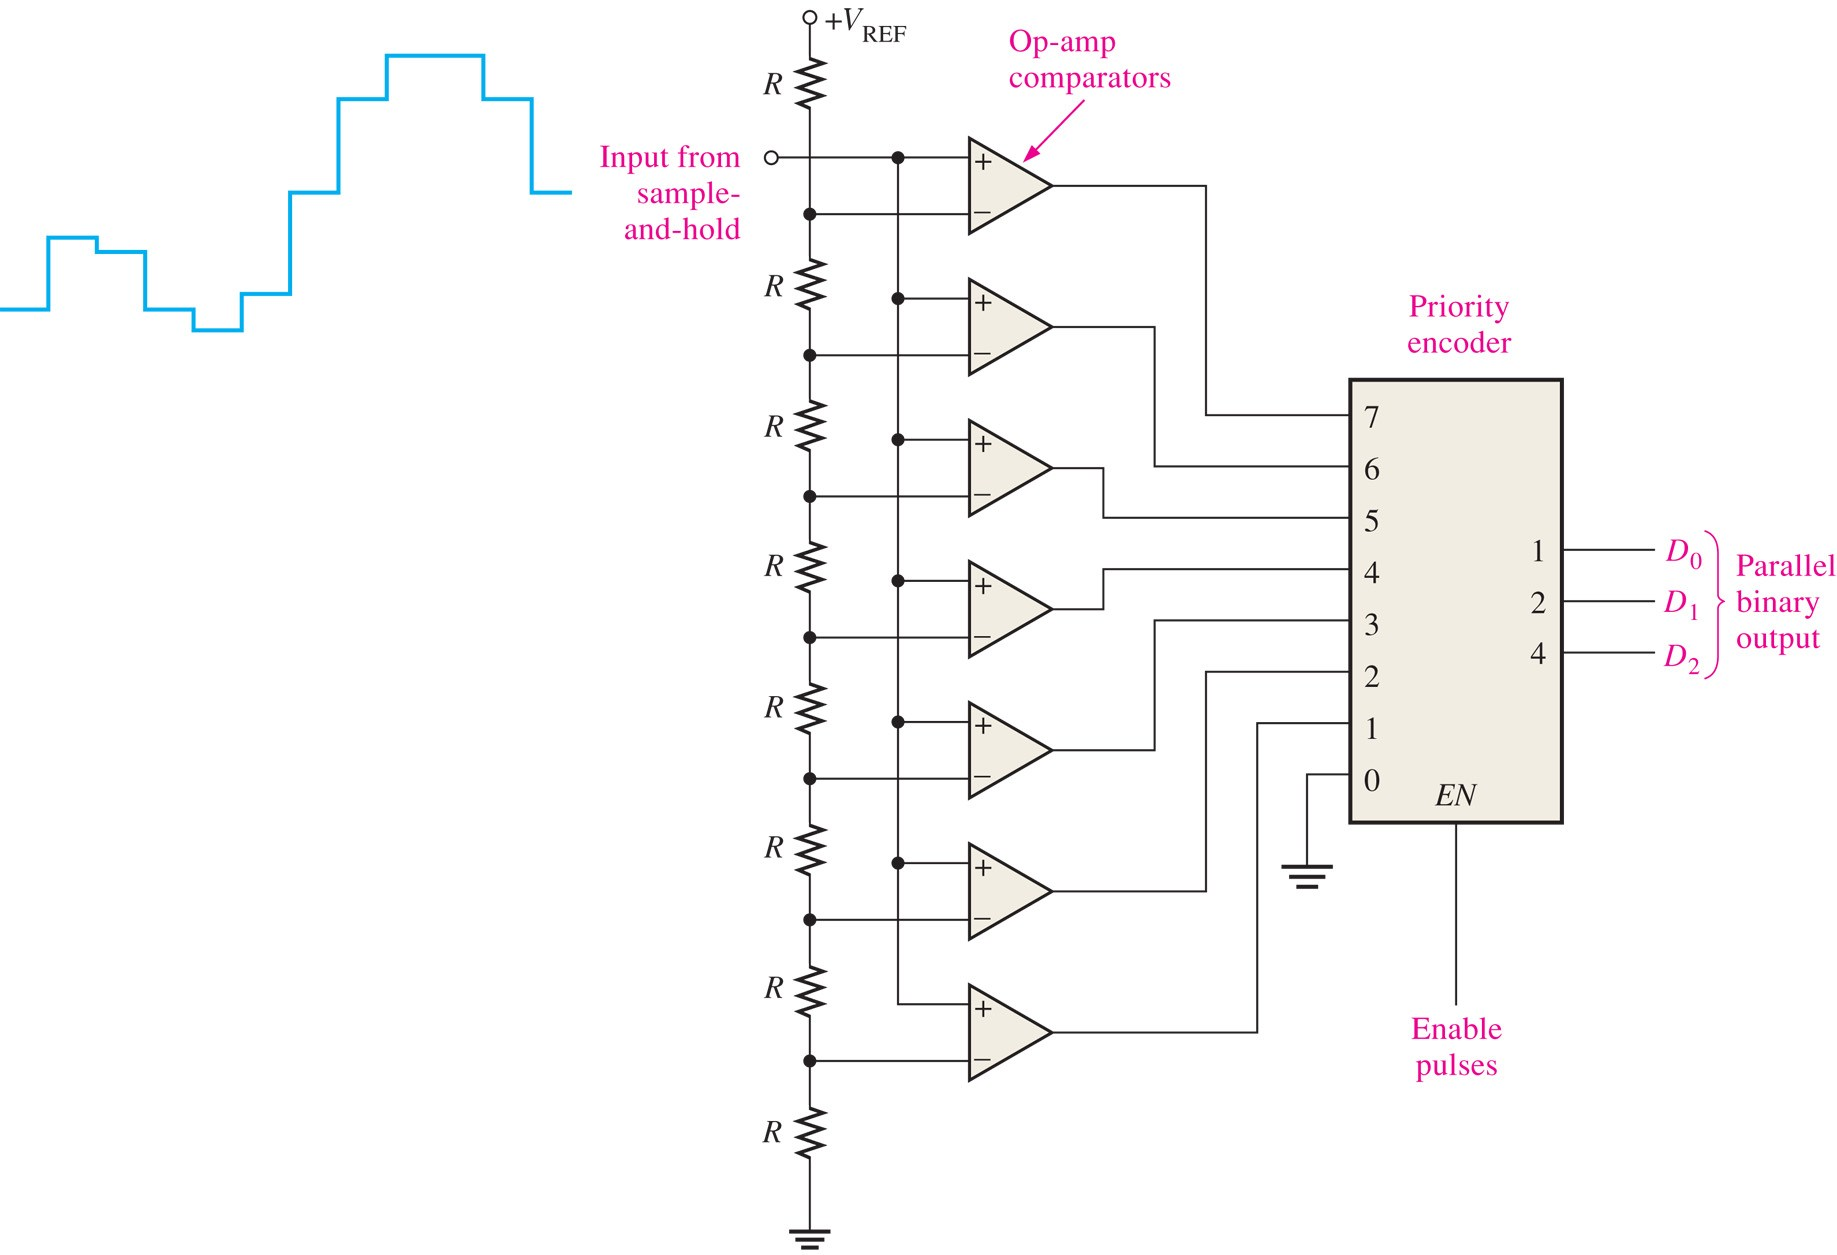
\includegraphics[width=0.55\textwidth]{figures/adc_6.jpg}
\caption{\label{fig:3} (Top) Op-amp comparator. (Bottom) 3-bit Flash ADC.}
\end{figure}
\end{frame}

\begin{frame}{Analog to Digital Conversion}
\begin{figure}
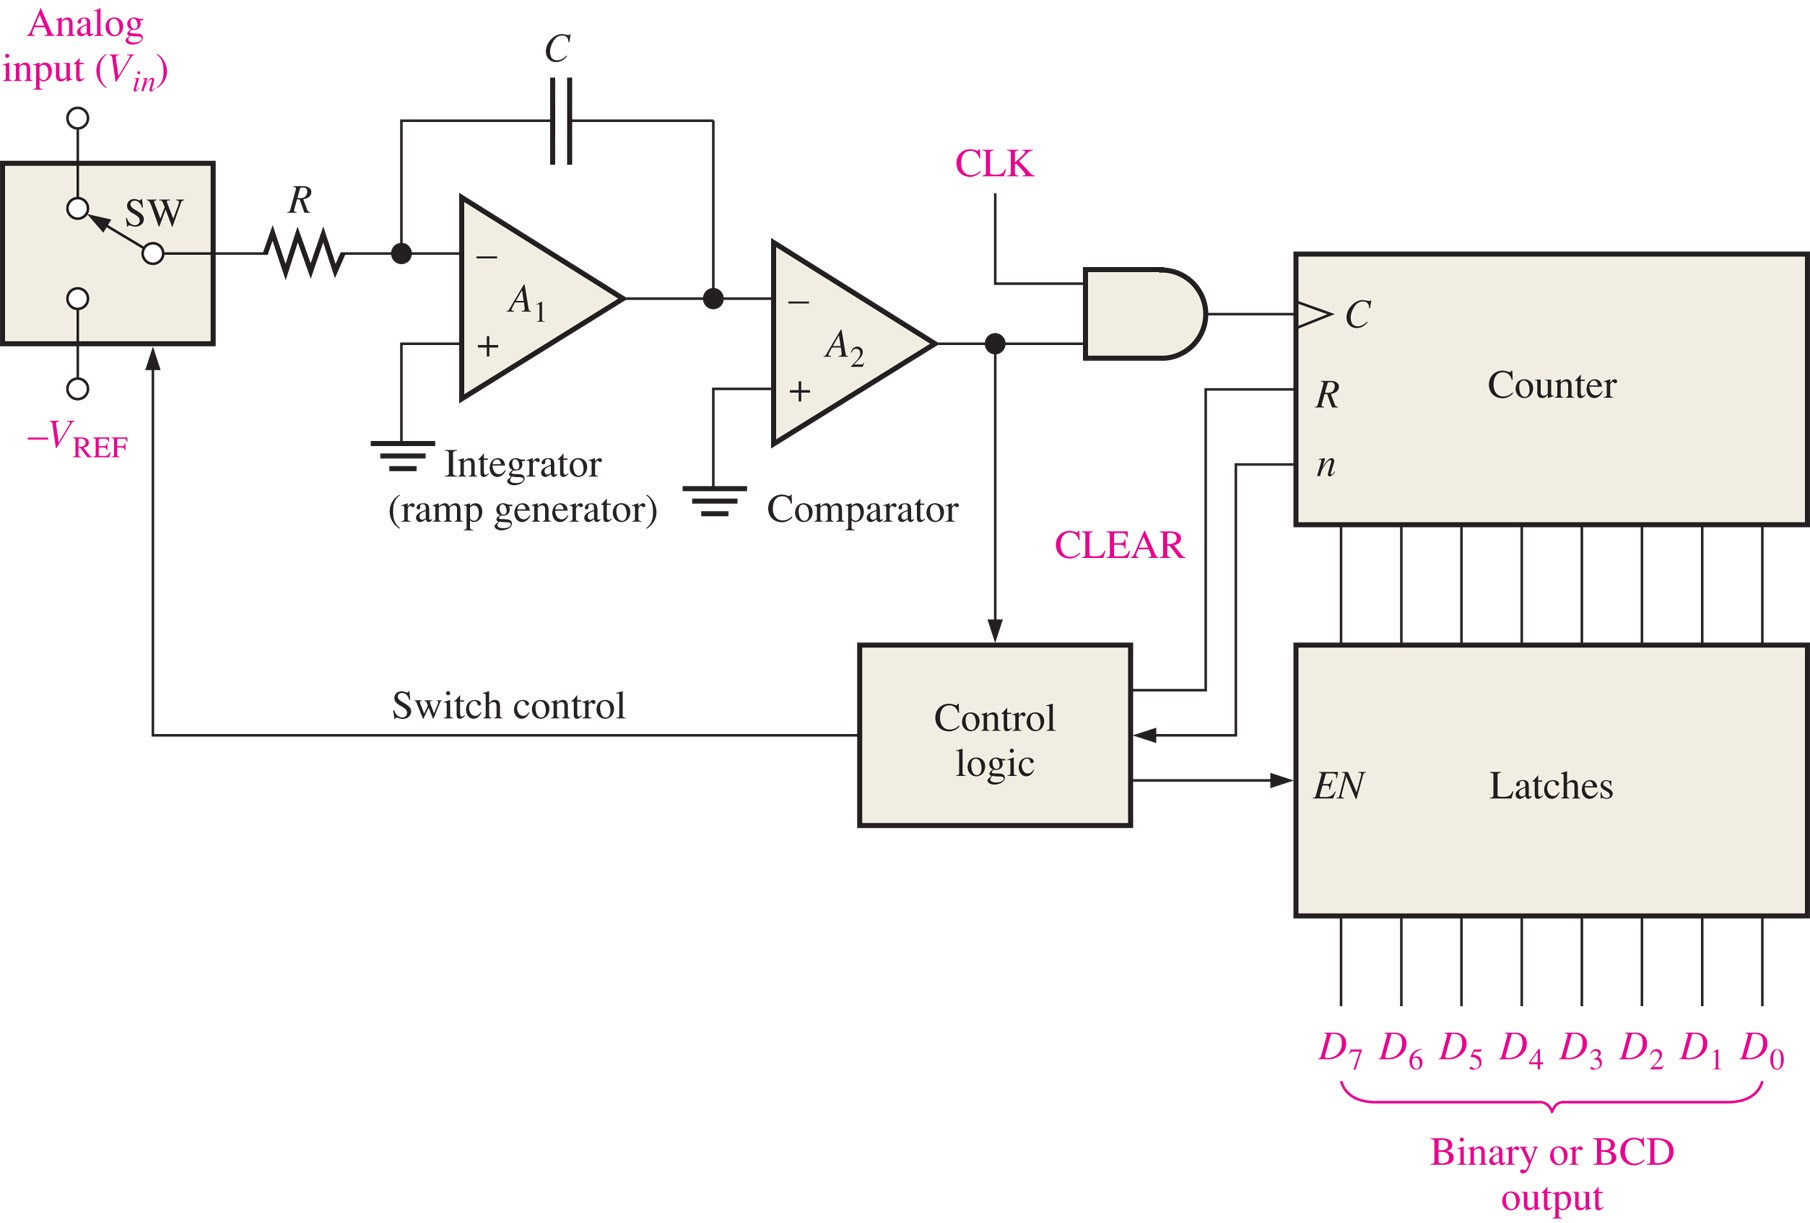
\includegraphics[width=0.75\textwidth]{figures/adc_8.jpg}
\caption{\label{fig:4} Dual slope ADC.}
\end{figure}
\end{frame}

\begin{frame}{Analog to Digital Conversion}
\begin{figure}
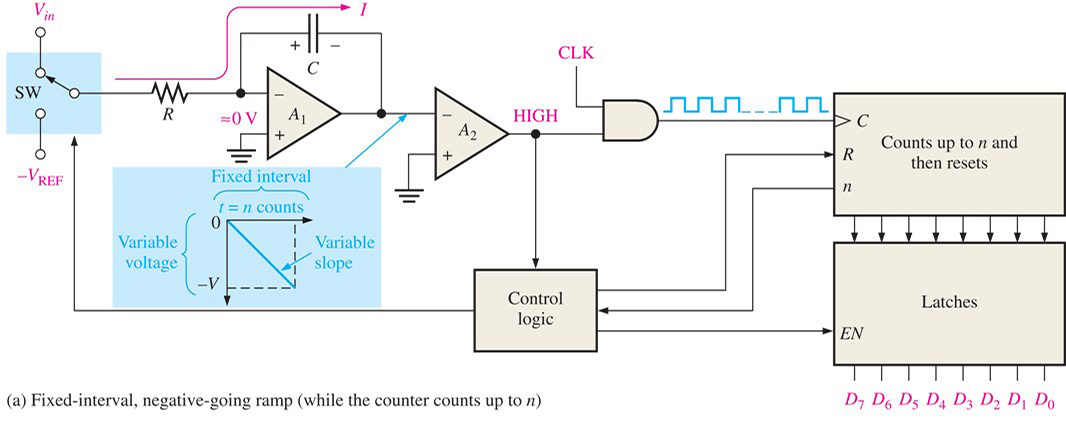
\includegraphics[width=0.75\textwidth]{figures/adc_9.jpg}
\caption{\label{fig:5} Dual slope ADC.}
\end{figure}
\end{frame}

\begin{frame}{Analog to Digital Conversion}
\begin{figure}
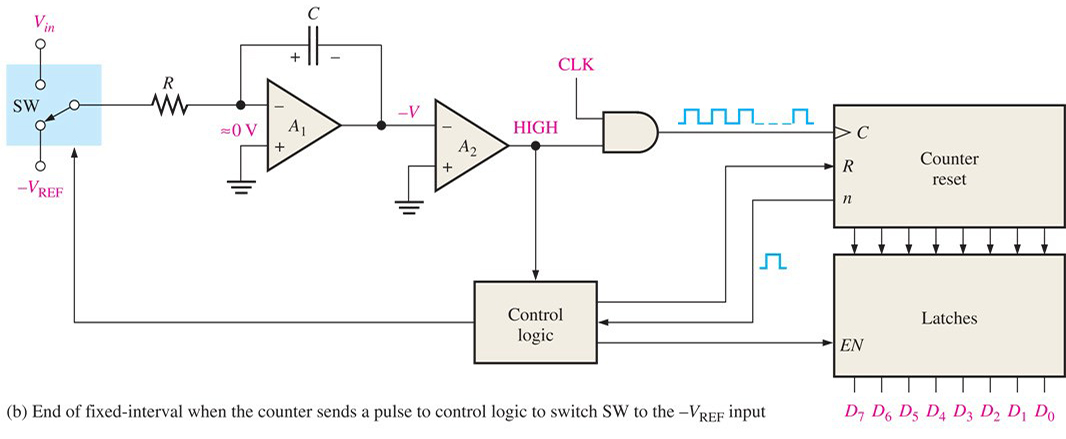
\includegraphics[width=0.75\textwidth]{figures/adc_10.jpg}
\caption{\label{fig:6} Dual slope ADC.}
\end{figure}
\end{frame}

\begin{frame}{Analog to Digital Conversion}
\begin{figure}
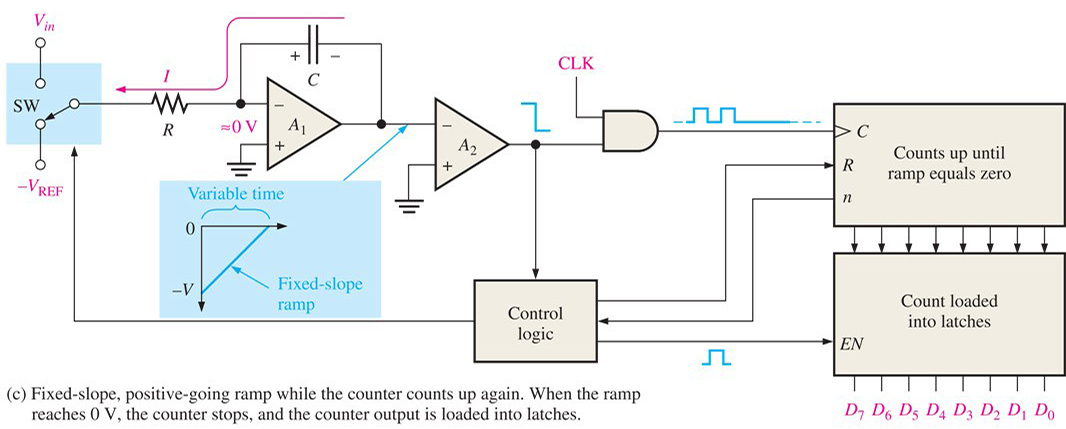
\includegraphics[width=0.75\textwidth]{figures/adc_11.jpg}
\caption{\label{fig:7} Dual slope ADC.}
\end{figure}
\end{frame}

\begin{frame}{Analog to Digital Conversion}
\begin{figure}
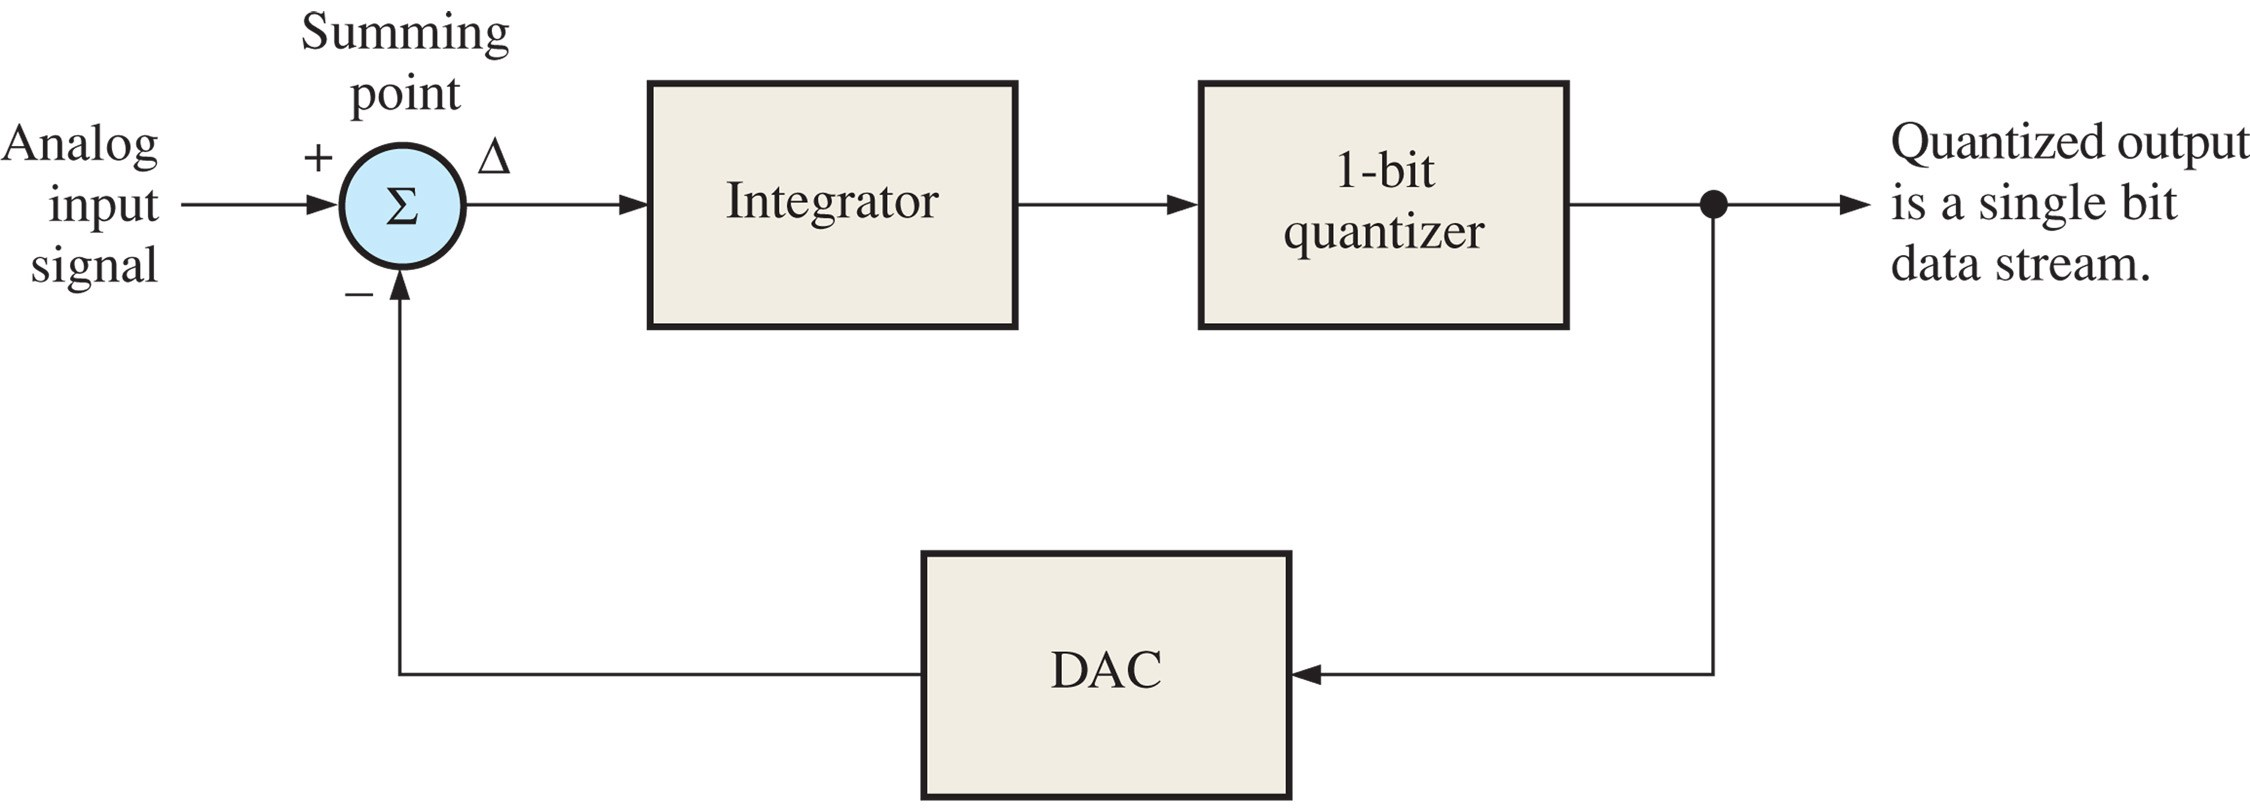
\includegraphics[width=0.55\textwidth]{figures/adc_12.jpg}
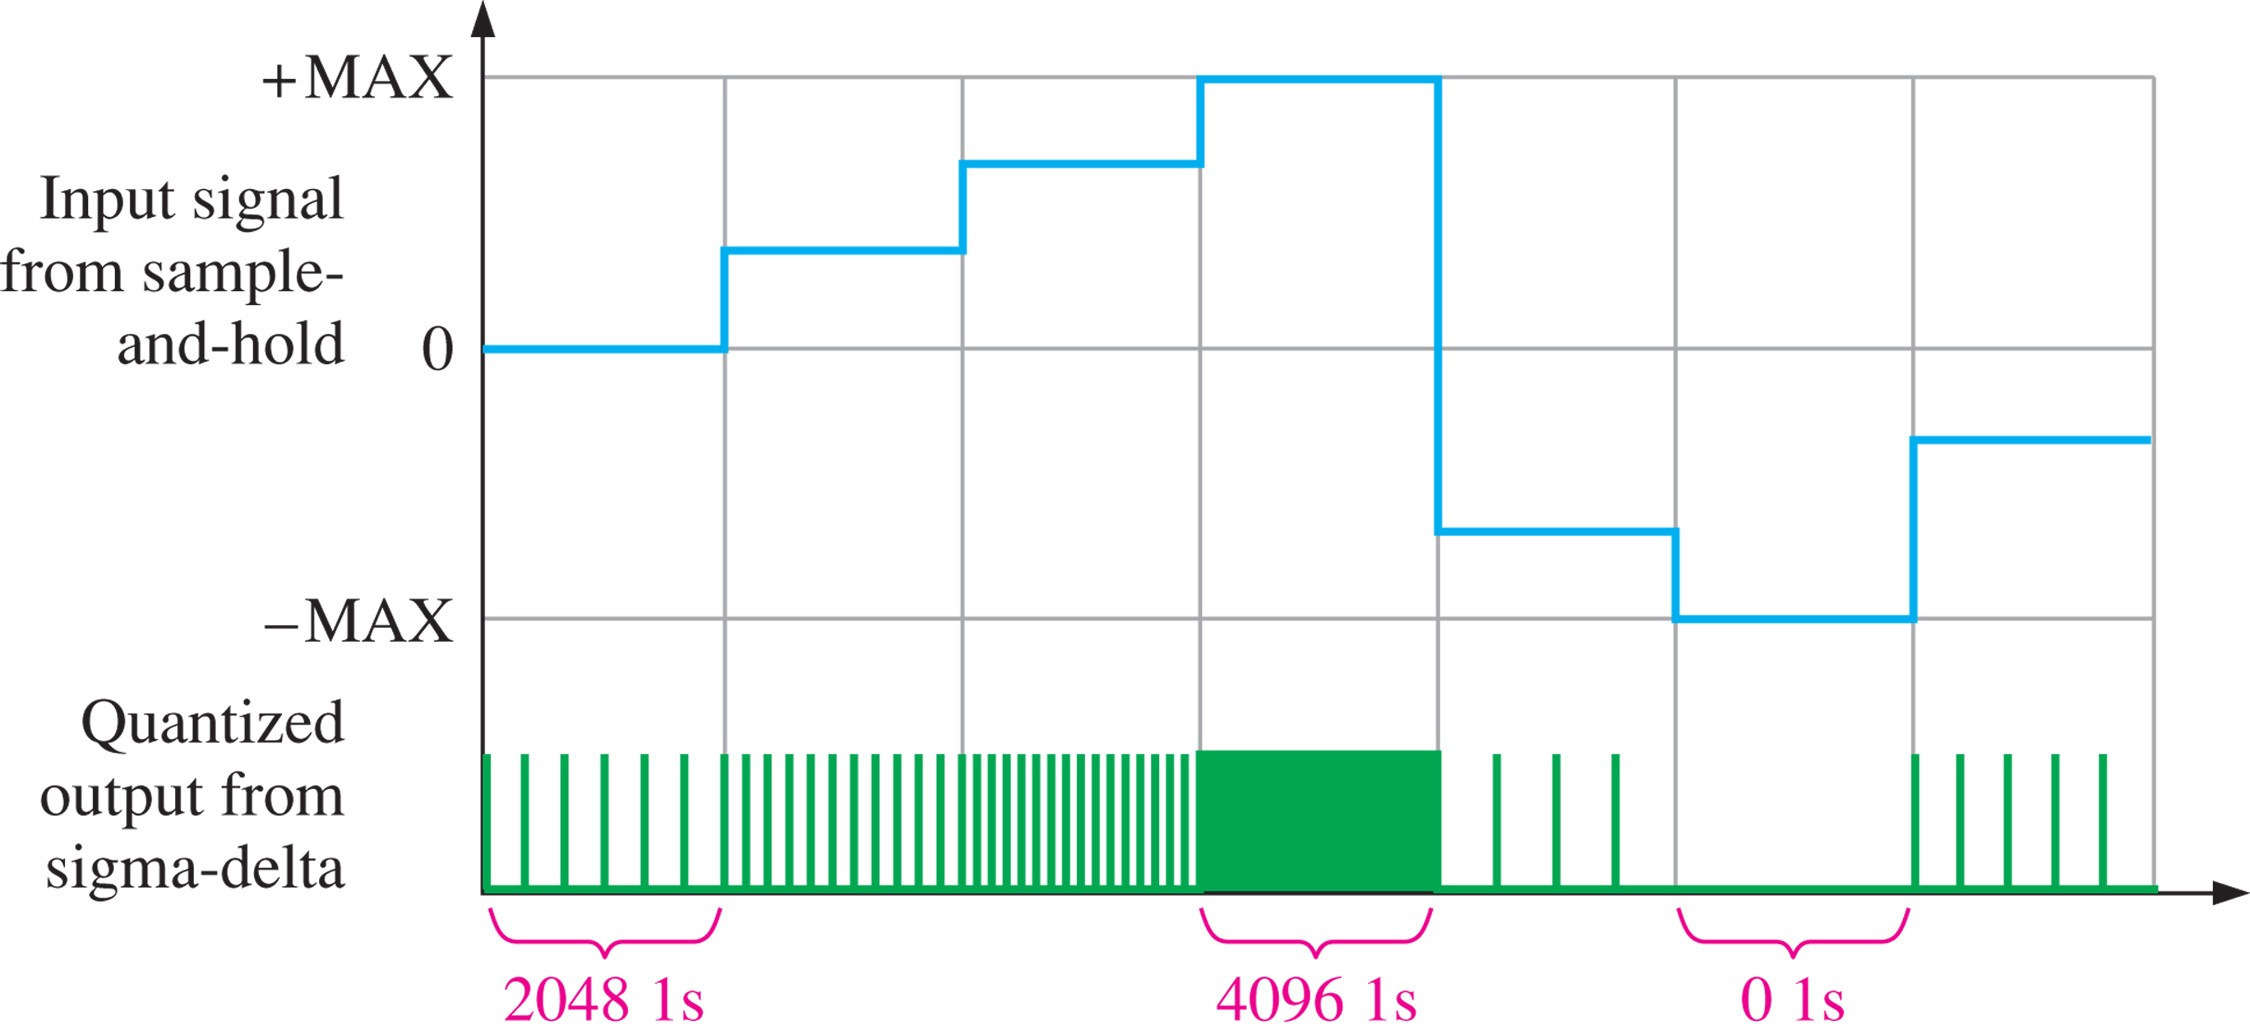
\includegraphics[width=0.55\textwidth]{figures/adc_13.jpg}
\caption{\label{fig:8} Sigma-Delta ADC.}
\end{figure}
\end{frame}

\begin{frame}{Analog to Digital Conversion}
\begin{figure}
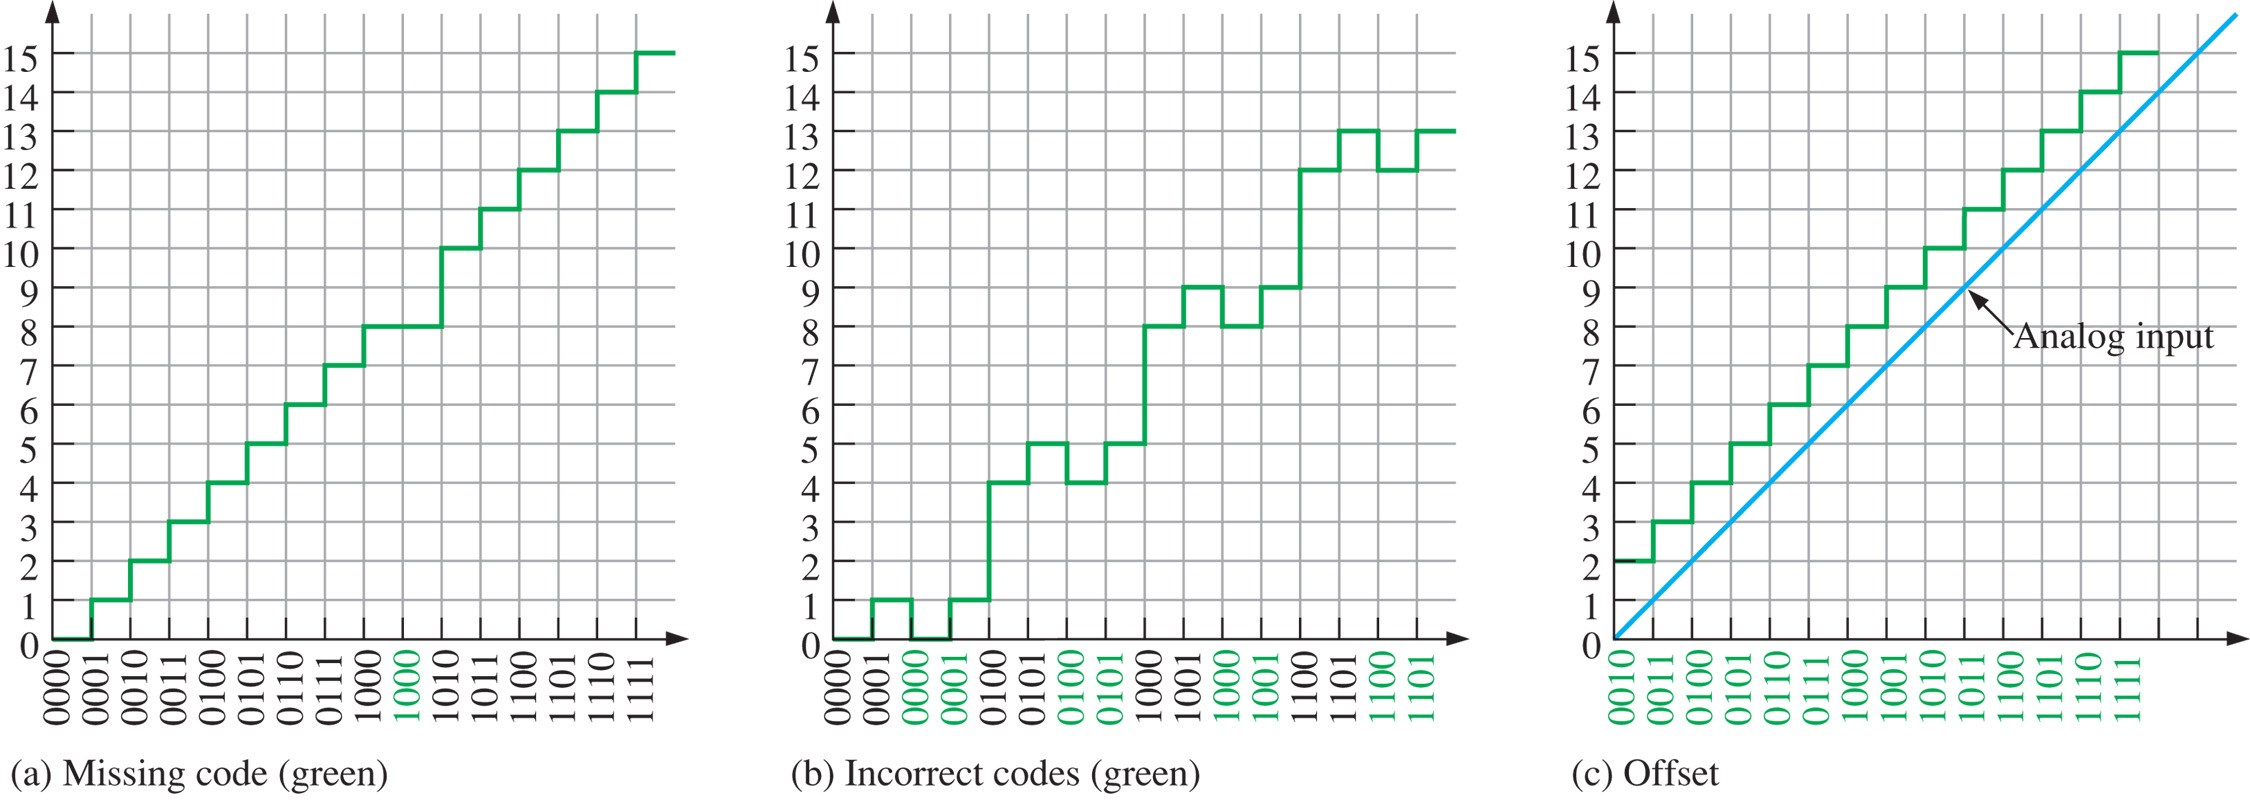
\includegraphics[width=0.75\textwidth]{figures/adc_14.jpg}
\caption{\label{fig:9} Types of ADC error.}
\end{figure}
\end{frame}

\begin{frame}{Analog to Digital Conversion}
\begin{figure}
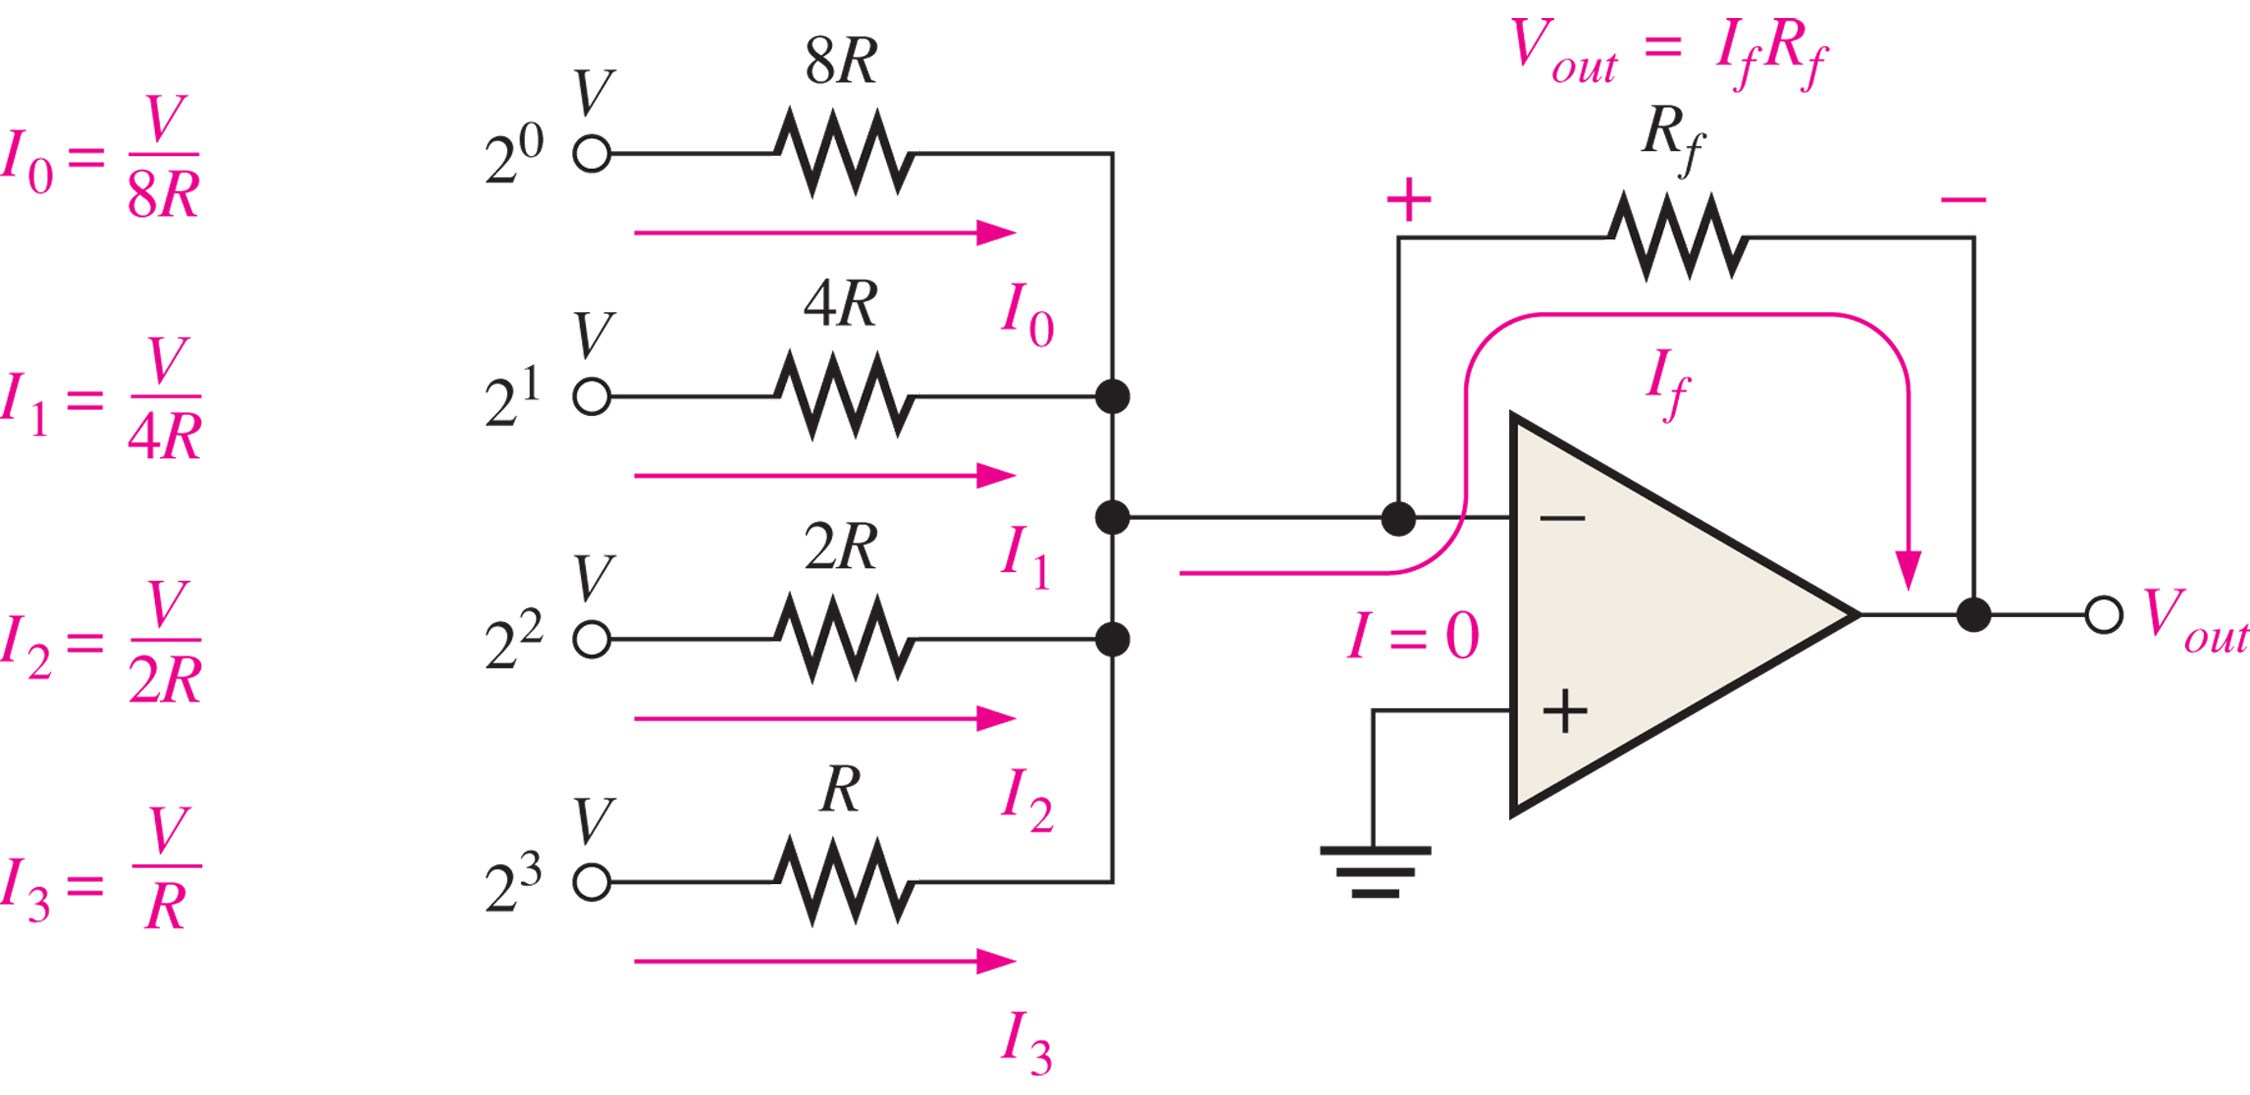
\includegraphics[width=0.75\textwidth]{figures/adc_15.jpg}
\caption{\label{fig:10} Binary-weighted DAC.}
\end{figure}
\end{frame}

\begin{frame}{Analog to Digital Conversion}
\begin{figure}
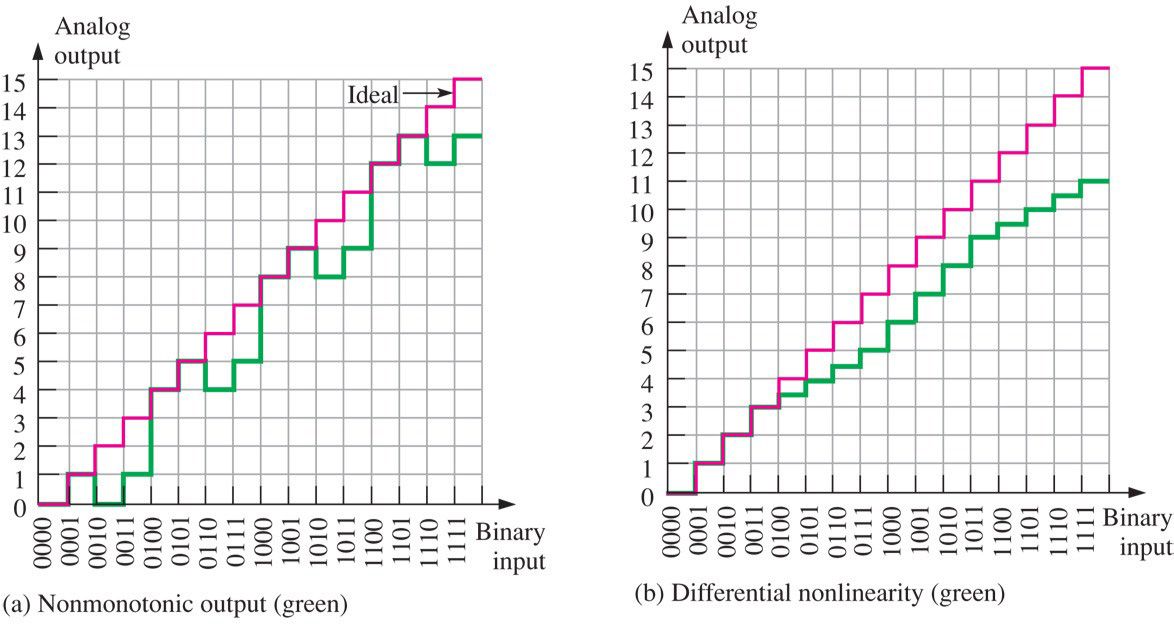
\includegraphics[width=0.55\textwidth]{figures/adc_16.jpg}
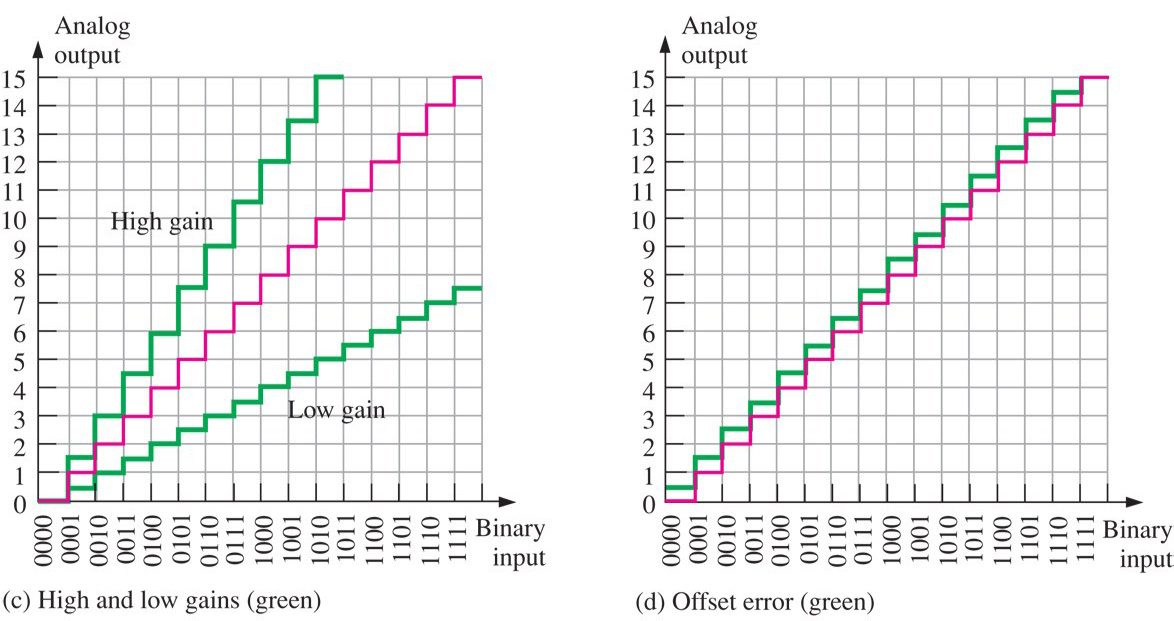
\includegraphics[width=0.55\textwidth]{figures/adc_17.jpg}
\caption{\label{fig:11} Types of DAC error.}
\end{figure}
\end{frame}

\section{Conclusion}

\begin{frame}{Unit 4 Summary}
\begin{enumerate}
\item Analog to Digital Conversion (ADC)
\item Digital to Analog Conversion (DAC)
\item Digital Signal Processing (DSP)
\item Digital Signal Processors
\end{enumerate}
\end{frame}

\end{document}
